\documentclass{beamer}

\usepackage[utf8]{inputenc}
\usepackage{default}
\usepackage{graphicx}


\makeatletter
\newcommand*{\rom}[1]{\expandafter\@slowromancap\romannumeral #1@}
\makeatother


% shows how to change default (blue) colours in the default beamer theme
% found here: http://joerglenhard.wordpress.com/tag/latex/
\definecolor{WaterlooRed}{RGB}{145,11,46}
\setbeamercolor{title}{fg=WaterlooRed}
\setbeamercolor{frametitle}{fg=WaterlooRed}
\setbeamercolor{structure}{fg=WaterlooRed}

% adds logo in the footer
\logo{
\includegraphics[scale=.25]{img/csuow}}

\title[]{Web Application Deployment Stages}
\author[Siming Sun, Xu Cui]{Siming Sun, Xu Cui}
\institute{
\includegraphics[scale=0.25]{img/UniversityOfWaterloo_logo_vert_rgb.png}}
\date{{\tiny\today}}

\begin{document}

\begin{frame}
  \titlepage
\end{frame}


\begin{frame}
  \frametitle{Agenda}
  \begin{itemize}
  \item Concepts
  \item Examples
  \item Summary
  \end{itemize}
\end{frame}


\begin{frame}
  \frametitle{Concept - High Overview}
  \begin{figure}
  	\centering
  	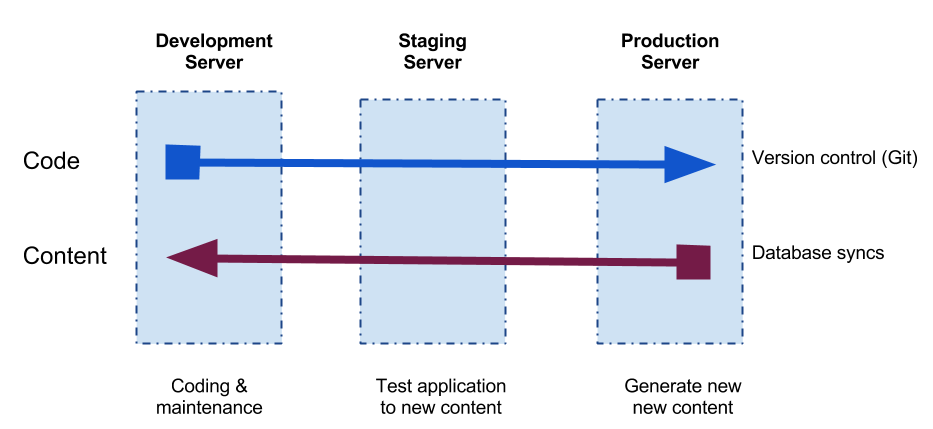
\includegraphics[scale=0.35]{img/Madhatter_presentation1_2.png}
  	\caption{Borrowed from \url{https://openconcept.ca/blog/mgifford/flow-content-code}}
  \end{figure}
\end {frame}


\begin{frame}
  \frametitle{Concepts - Deployment Stages}
  \begin{itemize}
  \item DEV: Working code copy. Changes made by developers are deployed here so integration and features can be tested. This environment is rapidly updated and contains the most recent version of the application.
  \item QA: (Not all companies will have this). Environment for quality assurance; this provides a less frequently changed version of the application which testers can perform checks against.
  \item staging: This is the release candidate, and this environment is normally a mirror of the production environment. The staging area contains the \"next\" version of the application and is used for final stress testing and client/manager approvals before going live.
  \item production: This is the currently released version of the application, accessible to the client/end users. This version preferably does not change except for during scheduled releases.
  \end{itemize}
\end{frame}


\begin{frame}
  \frametitle{Examples \rom{1}}
  \begin{figure}
  	\centering
  	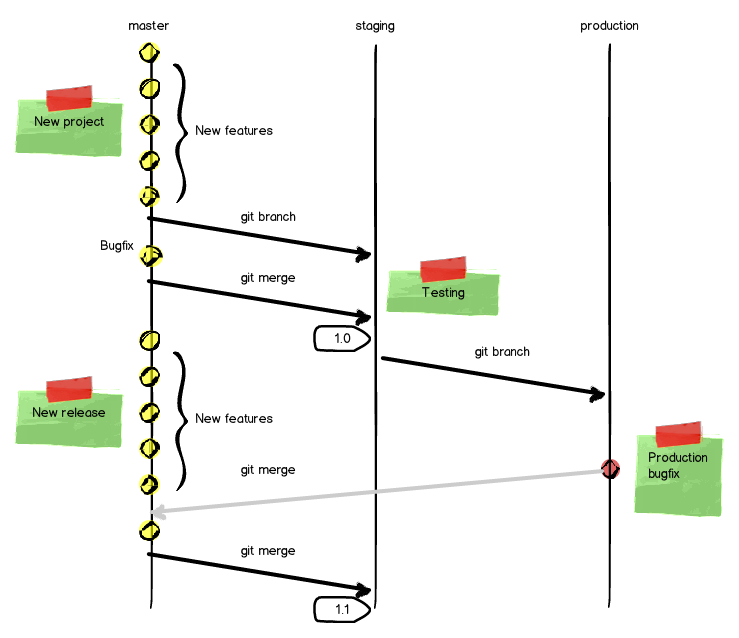
\includegraphics[scale=0.30]{img/madhatter_git-workflow.png}
  	\caption{Borrowed from a http://techblog.md-systems.ch/}
  \end{figure}
\end {frame}

\begin{frame}
  \frametitle{Examples \rom{2}}
  \begin{figure}
  	\centering
  	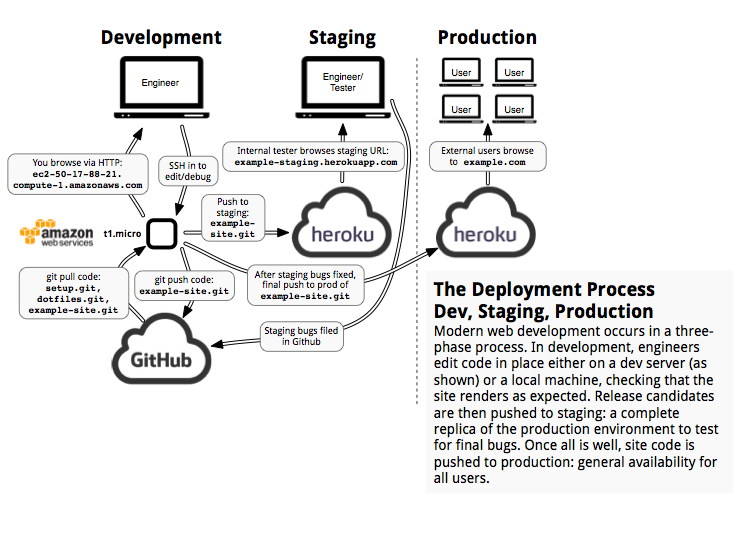
\includegraphics[scale=0.35]{img/madhatter_1.png}
  	\caption{Borrowed from a standford course - Startup Engineering}
  \end{figure}
\end {frame}



\begin{frame}
  \frametitle{Summary}
  \begin{itemize}
  \item What is good for MadHatter?
  \item Security control
  \item Who's responsible for which stage?
  \end{itemize}
\end {frame}

\end{document}

%
